
%%%%%%%%%%%%%%%%%%%%%%%%%%%%%%%%%%%%%%%%%%%%%%%%%%%%%%%%%%%%%%%%%%%%%%%%
% Evaluation
%%%%%%%%%%%%%%%%%%%%%%%%%%%%%%%%%%%%%%%%%%%%%%%%%%%%%%%%%%%%%%%%%%%%%%%%
\section{Experimental Study}
\label{sec:evaluation}

%-------plots------
\begin{table*}[!htbp]\footnotesize
\scriptsize
\begin{tabular}{lll}

%HOSP 
\begin{tikzpicture}
    \begin{axis}[
        legend pos=outer north east,        
        title=(a) \textsc{hosp} Data Cleaning for 90k,
        xlabel=noise,
        ylabel=F1, ]

         \addplot[mark=diamond] table[x=NOISE, y=CFDF1] {data/hosp-evaluation-90-datasize.tsv};
         \addplot table[x=NOISE, y=MDF1] {data/hosp-evaluation-90-datasize.tsv};
         \addplot table[x=NOISE, y=CFDMDF1] {data/hosp-evaluation-90-datasize.tsv};

        \legend{$cfd$,$md$,$cfd+md$},

    \end{axis}
\end{tikzpicture}
    &  
    

    \begin{tikzpicture}
%\selectcolormodel{gray}
   \begin{axis}[
       legend pos=outer north east,
       title=(b) \textsc{hosp} Data Cleaning for noise 10\%,
       xlabel=data size in k,
       ylabel=F1, ]

         \addplot[mark=diamond] table[x=DATASIZE, y=CFDF1] {data/hosp-evaluation-10-noise.tsv};
         \addplot table[x=DATASIZE, y=MDF1] {data/hosp-evaluation-10-noise.tsv};
         \addplot table[x=DATASIZE, y=CFDMDF1] {data/hosp-evaluation-10-noise.tsv};

       \legend{$cfd$,$md$,$cfd+md$},

   \end{axis}
\end{tikzpicture}
&
\begin{tikzpicture}
%\selectcolormodel{gray}
   \begin{axis}[
       legend pos=outer north east,
       title=(c) Runtime for \textsc{hosp} Data Cleaning,
       xlabel=data size in k,
       ylabel=seconds, ]

         \addplot[mark=diamond] table[x=DATASIZE, y=TIME] {data/hosp-evaluation-2-noise.tsv};
         \addplot table[x=DATASIZE, y=TIME] {data/hosp-evaluation-4-noise.tsv};
         \addplot table[x=DATASIZE, y=TIME] {data/hosp-evaluation-6-noise.tsv};
         \addplot table[x=DATASIZE, y=TIME] {data/hosp-evaluation-8-noise.tsv};
         \addplot table[x=DATASIZE, y=TIME] {data/hosp-evaluation-10-noise.tsv};

       \legend{$noise 2$,$noise 4$,$noise 6$,$noise 8$,$noise 10$},

   \end{axis} 
   \end{tikzpicture}

 \\
%TPC-H results

\begin{tikzpicture}
%\selectcolormodel{gray}
  \begin{axis}[
      legend pos=outer north east,
      title=(d) \textsc{tpc-h} Data Cleaning for 20k,
      xlabel=noise,
      ylabel=F1, ]

         \addplot[mark=diamond] table[x=NOISE, y=CFDF1] {data/tpch-eval-20000-datasize.tsv};
         \addplot table[x=NOISE, y=MDF1] {data/tpch-eval-20000-datasize.tsv};
         \addplot table[x=NOISE, y=CFDMDF1] {data/tpch-eval-20000-datasize.tsv};

      \legend{$cfd$,$md$,$cfd+md$},

  \end{axis}
\end{tikzpicture}

& \begin{tikzpicture}
%\selectcolormodel{gray}
  \begin{axis}[
      legend pos=outer north east,
      title=(e) \textsc{tpc-h} Data Cleaning for noise 2\%,
      xlabel=data size,
      ylabel=F1, ]

         \addplot[mark=diamond] table[x=DATASIZE, y=CFDF1] {data/tpch-eval-2-noise.tsv};
         \addplot table[x=DATASIZE, y=MDF1] {data/tpch-eval-2-noise.tsv};
         \addplot table[x=DATASIZE, y=CFDMDF1] {data/tpch-eval-2-noise.tsv};

      \legend{$cfd$,$md$,$cfd+md$},

  \end{axis}
\end{tikzpicture} & 

\begin{tikzpicture}
%\selectcolormodel{gray}
  \begin{axis}[
      legend pos=outer north east,
      title=(f) Runtime for TPCH Data Cleaning,
      xlabel=data size,
      ylabel=seconds, ]

         \addplot[mark=diamond] table[x=DATASIZE, y=TIME] {data/tpch-evaluation-2-noise.tsv};
         \addplot table[x=DATASIZE, y=TIME] {data/tpch-evaluation-4-noise.tsv};
         \addplot table[x=DATASIZE, y=TIME] {data/tpch-evaluation-6-noise.tsv};
         \addplot table[x=DATASIZE, y=TIME] {data/tpch-evaluation-8-noise.tsv};
         \addplot table[x=DATASIZE, y=TIME] {data/tpch-evaluation-10-noise.tsv};

      \legend{$noise 2$,$noise 4$,$noise 6$,$noise 8$,$noise 10$},

  \end{axis}
\end{tikzpicture}
\end{tabular}
\caption{\label{tab:plots} Evaluation of the data repair method based on Markov logic applied on the ~\textsc{hosp} and~\textsc{tpc-h} datasets. (a)-(c) Data repair on \textsc{hosp} with an extended Markov logic method. (d)-(f) Experimental study of the Markov logic data cleaning on synthetic dataset \textsc{tpc-h}.}
\end{table*}


\begin{table}[t]\footnotesize
%\scriptsize
\centering
\begin{tabular}{@{}cccc@{}}
\toprule
{\bf dataset}       & 
{\bf \begin{tabular}[c]{@{}c@{}}numer \\ of tuples\end{tabular}} & 
{\bf \begin{tabular}[c]{@{}c@{}}number\\ of formulas\end{tabular}}  & 
{\bf \begin{tabular}[c]{@{}c@{}}runtime\\ (sec)\end{tabular}} \\ 
                                                         \\
\midrule
                     & 63K                                                                                                                     & 21                                                                                                                                        & 242                                                           \\
{\bf \textsc{hosp}}           & 83K                                                                                                                      & 21                                                                                                                                        & 477                                                           \\
\multicolumn{1}{l}{} & 143K                                                                                                                    & 21                                                                                                                                        & 1107                                                          \\ \midrule
\multicolumn{1}{l}{} & 20K                                                                                                                      & 15                                                                                                                                        & 41                                                            \\
{\bf \textsc{tpc-h}}           & 40K                                                                                                                      & 15                                                                                                                                        & 131                                                           \\
\multicolumn{1}{l}{} & 100K                                                                                                                     & 15                                                                                                                                        & 732                                                           \\ \bottomrule
\end{tabular}
\caption{\label{tab:runtime} Scalability of the data cleaning for \textsc{tpc-h} and \textsc{hosp} datasets (with fixed noise 4\%). }
\end{table}


\begin{table*}[t]\footnotesize
\scriptsize
\centering
\begin{tabular}{@{}llll@{}}
\toprule
& \multicolumn{1}{c}{\textsc{hosp}}  & \multicolumn{1}{c}{\textsc{tpc-h}}  & \multicolumn{1}{c}{\textsc{msag}}  \\ \midrule
\begin{tabular}[c]{@{}l@{}}
 observed\\ predicates
\end{tabular} 
& 
\begin{tabular}[c]{@{}l@{}}
\textsl{providerNr/\textsc{hosp}}(hid, pn)\\ 
\textsl{hospitalName/\textsc{hosp}}(hid, n)\\ 
\textsl{address/\textsc{hosp}}(hid, add)\\ 
\textsl{city/\textsc{hosp}}(hid, c)\\ 
\textsl{state/\textsc{hosp}}(hid, st)\\ 
\textsl{zipCode/\textsc{hosp}}(hid, code)\\ 
%\textsl{countryName/\textsc{hosp}}(hid, country)\\ 
\textsl{phoneNumber/\textsc{hosp}}(hid, numb)\\ 
\textsl{condition/\textsc{hosp}}(hid, cond)\\ 
\textsl{measureCode/\textsc{hosp}}(hid, mcode)\\ 
%\textsl{measureName/\textsc{hosp}}(hid, mname)\\ 
\textsl{score/\textsc{hosp}}(hid, score)\\ 
\textsl{zip/\textsc{zipcode}}(zid, code)\\ 
\textsl{state/\textsc{zipcode}}(zid, st)
\end{tabular}                       
& 
\begin{tabular}[c]{@{}l@{}}
\textsl{custKey}(id, key)\\ 
\textsl{name}(id, n)\\ 
\textsl{addr}(id, add)\\ 
\textsl{natKey}(id, nkey)\\ 
\textsl{phone}(id, ph)\\ 
\textsl{acc}(id, a)\\ 
\textsl{mrkt}(id, m)\\ 
\textsl{orderKey}(id, okey)\\ 
%\textsl{orderStatus}(id, st)\\ 
\textsl{totalPrice}(id, p)\\ 
\textsl{orderDate}(id, d)\\ 
\textsl{orderPriority}(id, pr) \\ 
\textsl{clerk}(id, c)
\end{tabular} 
& 
\begin{tabular}[c]{@{}l@{}}
\textsl{publishYear}(paperid, pubyear)\\
\textsl{author}(paperid, authorid)\\
\textsl{affiliation}(paperid, affilid)\\
\textsl{inRange}(pubyear, pubyear)\\
\textsl{originAffiliationName}(affilid, oname)\\
\textsl{normalAffiliationName}(affilid, nname)
\end{tabular}
\\ \midrule % now hidden predicates
\begin{tabular}[c]{@{}l@{}}
hidden \\ predicates
\end{tabular}  
& \begin{tabular}[c]{@{}l@{}}
  \textsl{equal-HospitalName/\textsc{hosp}}(hid, hid)\\ 
  \textsl{equal-Address/\textsc{hosp}}(hid, hid)\\ 
  \textsl{equal-City/\textsc{hosp}}(hid, hid)\\ 
  \textsl{equal-State/\textsc{hosp}}(hid, hid)\\ 
  \textsl{equal-ZipCode/\textsc{hosp}}(hid, hid)\\ 
  %\textsl{equal-CountryName/\textsc{hosp}}(hid, hid)\\ 
  \textsl{equal-PhoneNumber/\textsc{hosp}}(hid, hid)\\ 
  %\textsl{equal-MeasureName/\textsc{hosp}}(hid, hid)\\ 
  \textsl{equal-Condition/\textsc{hosp}}(hid, hid)\\ 
  \textsl{\textsc{hosp}/match-State/\textsc{ZipCode}}(hid, zid)\\ 
  \textsl{\textsc{hosp}/match-ZipCode/\textsc{ZipCode}}(hid, code)
\end{tabular} 
& 
\begin{tabular}[c]{@{}l@{}}
 \textsl{equal-Names}(id, id)\\ 
 \textsl{equal-Addr}(id, id)\\ 
 \textsl{equal-Natkey}(id, id)\\ 
 \textsl{equal-Phone}(id, id)\\ 
 \textsl{equal-Acc}(id, id)\\ 
 \textsl{equal-Mrkt}(id, id)\\ 
 \textsl{match-Phone}(id, id)\\ 
 \textsl{match-Addr}(id, id)
\end{tabular} 
& 
\begin{tabular}[c]{@{}l@{}}
\textsl{equal-Affiliation}(paperid, paperid)\\
\textsl{equal-OriginNames}(oname, oname)\\
\textsl{equal-OriginNamesByPaperId}(paperid, paperid)\\
\textsl{equal-NormalNames}(nname, nname)\\
\textsl{equal-NormalNamesByPaperId}(paperid, paperid)\\
\textsl{missingOriginName}(paperid, oname)
\end{tabular}\\ \bottomrule
\end{tabular}
\caption{\label{tab:predicates} Markov logic predicates used in data quality rules.}
\end{table*}

\begin{table}[t]\footnotesize
%\scriptsize
\centering
\begin{tabular}{ccc}
\textbf{\textit{Paper}}         & \textbf{\textit{Author}}     & \textbf{\textit{Organization}}      \\ \hline
\textsl{paper\_id}     & \textsl{author\_id} & \textsl{affiliation\_id}  \\
\textsl{publish\_year} &            & \textsl{origin\_name}     \\
              &            & \textsl{normalized\_name}\\ \hline
\end{tabular}
\caption{Entities \textbf{\textit{Paper}}, \textbf{\textit{Author}} and \textbf{\textit{Organization}} and their attributes that have been used in experiments for Web data cleaning with Markov logic.}
    \label{tab:msagattrs}
\end{table}

We evaluate our method through an experimental study on well-known datasets, which have been used for assessing other data cleaning systems~\cite{Dallachiesa:2013:NCD:2463676.2465327, chu2013holistic, llunaticVDLB2013b, bohannon2005cost}. Each of these datasets suffers from different data quality issues such as duplicates, inconsistency, or missing values. 

\subsection{Experimental Setting} 
We conduct our experiments on the following real-life and synthetic datasets.

%\todo[inline]{make our data public}

\textbf{\textsc{hosp}}. The \textsc{hosp} dataset has been published by the US Department of Health $\&$ Human Services\footnote{http://www.medicare.gov/hospitalcompare/Data/Data-Download.html}. This dataset comprises 9 attributes: \textsl{addr}, \textsl{city}, \textsl{cond}, \textsl{country}, \textsl{hospname}, \textsl{measure}, \textsl{phone}, \textsl{state}, \textsl{zip}. 
We use 6 CDFs and one MD, which have been manually designed. These data quality rules have been generously provided to us by the researchers Dallachiesa et al. from~\cite{Dallachiesa:2013:NCD:2463676.2465327}. One example of their rules is a CFD that states that if two tuples of \textsc{hosp} match on attribute values for $\textsl{zip}$, then they should also match on \textsl{country} and \textsl{state} attribute values. They define an MD that makes use of another table, namely US ZIP codes: ZIPCode\footnote{http://databases.about.com/od/access/a/zipcodedatabase.htm}. This additional dataset contains $43K$ tuples with two attributes: \textsl{zip} and \textsl{state}. The MD defines that if two tuples from \textsl{hosp} and ZIPCode possess the same zip code values, and the state values are distinct, then the state value from the ZIPCode table should be adopted. 

\textbf{\textsc{tpc-h}.} The \textsc{tpc-h}\footnote{http://www.tpc.org/tpch/} dataset is well-known dataset used in decision support benchmarks for databases. For our experiments we use two relations, \textit{Customer} and \textit{Orders}, which we join in order to introduce duplications on the \textit{Customer} relations data. The resulting dataset consists of 17 attributes of schema $T$: \textsl{c\_custkey}, \textsl{c\_name}, \textsl{c\_address},  \textsl{c\_nationkey}, \textsl{c\_phone}, \textsl{c\_acctbal},\\ \textsl{c\_mtksegment}, \textsl{c\_comment}, \textsl{o\_orderkey}, \textsl{o\_custkey},\\ \textsl{o\_orderstatus}, \textsl{o\_totalprice}, \textsl{o\_orderdate},\\ \textsl{o\_orderpriority}, \textsl{o\_clerk}, \textsl{o\_shippriority}, \textsl{o\_comment}. 

\textbf{Dirty Data.} We introduce noise into the relational datasets \textsc{hosp} and \textsc{tpc-h} to produce dirty data. Our methods handles several kinds of noise: missing values, errors from the active domain, and typos. We consider the initial data to be clean and therefore use it as ground truth. Additionally, we manually assess that the ground truth datasets are consistent with respect to the CFDs and MDs. Afterwards, we insert noise into the datasets. We conduct our experiments on the two datasets with different noise rates ranging from $\mathsf{noi\%}$=2$\%$ to $\mathsf{noi\%}$=10$\%$. We introduce this noise into different dataset sizes ranging from one thousand to one hundred thousand data points. The noise rate depicts the ratio of the number of erroneous values to the total number of values in the dataset. We only introduce noise to the attributes which are involved in data quality rules.

\textbf{\textsc{microsoft academic graph (msag)}.} Data quality issues are massively present in the context of the web due to the integration of heterogeneous data from different sources. Thus we include a third dataset - \textsc{microsoft academic graph (MSAG)}\footnote{http://research.microsoft.com/en-us/projects/mag/}~\cite{msag2015} - to assess our method on web data cleaning. MSAG is a heterogeneous entity graph comprised of six types of entities that model real-life academic relationships: field of study, author, institution, paper, venue, and conference instances. The raw data has been obtained from different sources (academic publishers and web-pages indexed by Bing search engine) and is organized in the form of a connected graph schema. For our experiments, we select three entities from the whole graph: \textit{author}, \textit{organization} and \textit{paper} entities. This part of \textsc{MSAG} is of interest because it reveals important characteristics of the extracted web data, such as missing and inconsistent values. In particular, we discover that there are inconsistencies in organization names for the same author. Furthermore, a number of entries suffer from missing affiliation by an author. In order to model and run data cleaning on this web dataset, we consider the attributes of the selected entities in \textsc{MSAG}, as presented in Table~\ref{tab:msagattrs}. 

\textbf{Data Quality Issues.} We extract a subset of complete entity instances in order to perform data cleaning experiments on web data. We reproduce data quality issues that we observe in \textsc{MSAG}: namely missing values. In order to a create gold standard to assess our data cleaning method, we proceed in the following way: We remove one affiliation entry from each author if there are more than three publications made by the same affiliation. Thus, we create a dataset with missing \textsl{affiliation\_id}, \textsl{origin\_name}, and \textsl{normalized\_name} attributes. We thereby obtain graph data where $37\%$ of all authors have one missing edge to theirs affiliation; $27\%$ are missing two edges for theirs institutions; $15\%$ miss three edges. Almost $21\%$ of authors suffer from missing more than three edges. 

\begin{figure}[t]
    \centering
    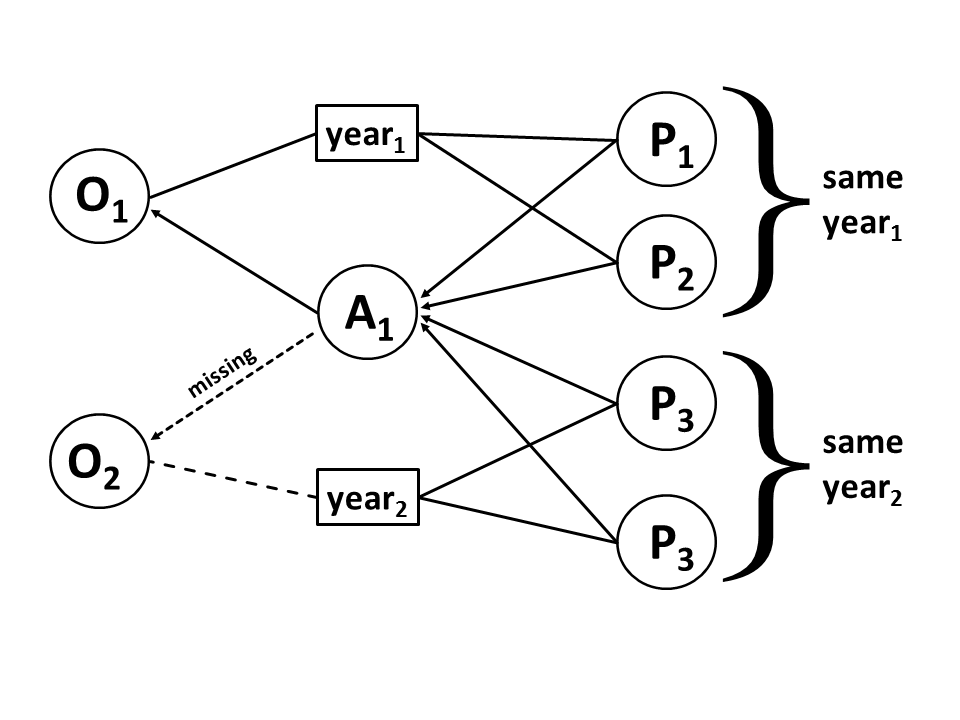
\includegraphics[width=0.25\textwidth, trim = 0mm 4mm 0mm 5mm, clip]{img/graph01.png}
    \caption{The part of the \textsc{msag} dataset illustrating missing organization values. Markov logic allows us to capture the following evidence: if two papers of the same author have been published in the same year, then they may be published by the author of the same organization. Nodes notation: A - denotes \textit{Author} entity; O - \textit{Organization} and P - \textit{Paper} entities. Missing edges are marked as dashed lines.}
    \label{fig:msagmissing}
\end{figure}

\textbf{Evaluation metrics.} We evaluate the effectiveness of our data cleaning method with a focus on two aspects: the accuracy and the performance of the method. To assess the accuracy of the data cleaning framework on relational data, we use \textit{Precision ($P$)}, \textit{Recall ($R$)}, and \textit{F-measure ($F_1$)}. We acquire master data (referred to as \textit{gold standard}), which is clean and correct. We assess the efficiency of our method by running experiments on datasets of different sizes ranging from one thousand to one hundred thousand tuples each. We leverage a state-of-the-art inference engine for Markov logic called \textit{RockIt}~\cite{NoessnerNS13} and the Gurobi solver version 5.6.3. All our experiments apply MAP inference for statistical relational learning. We execute the experiments on a Linux server with an Intel 3.4GHz 4 Cores CPU and 16 GB of RAM.
\\
\\
\\


\subsection{Holistic Data Cleaning: Deduplication and Accuracy}
\label{subsec:exp1}
%%%%%%%%%%%
In this experiment, we show that capturing the data issue interaction increases the overall accuracy in data cleaning. In particular, we study the connection between deduplication and improved data accuracy. We evaluate the accuracy of our method on different noise rates and different dataset sizes. We introduce noise by adding either typos or replacing values of attributes (active domain errors). We do not distinguish between these two kinds of errors. Table~\ref{tab:plots} shows the results of using Markov logic programs for data cleaning. The plots (a)-(c) illustrate the results for \textsc{hosp}, while plots (d)-(f) depict the results for \textsc{tpc-h}. %\note{DONT MAKE READERS THINK: Explain what readers see in these plots!!!} done.

In the first series of experiments, we fix the size for \textsc{hosp} and \textsc{tpc-h} to $90$K respectively $20$K tuples, while varying the noise rate from $2\%$ to $10\%$. The $x$-axis in Table~\ref{tab:plots} (a) and (d) represents the noise rate, the $y$-axis shows the corresponding $F_1$ measure values. First, we compare the results of separate executions of CDFs and MDs. After that we re-run the experiments with combined CFDs and MDs. When CFDs and MDs are modeled together in a single model for identifying dirty data, they are treated jointly and hence our method automatically picks the order of the data quality rules execution. The provided results in Table~\ref{tab:plots} (a) and (d) clearly demonstrate that jointly modeling CDFs and MDs improves the overall result because joint execution involves two processes simultaneously: matching (for values deduplication) and repair (for erroneous values). For this reason repairing supports matching, and by identifying matches we are able to fix erroneous values.

In particular, the low $F_1$ score of MDs in Table~\ref{tab:plots} (a)-(b) and (d)-(e) results from low precision and high recall. However, By adding CFDs to MDs the overall $F_1$ score improves. The counterintuitive upward trend of the $F_1$ values while increasing noise in Table~\ref{tab:plots} (a) and (d) results from the \textit{cutting plane inference} (CPI) \cite{riedel08improving} behavior. In all experiments, we use the CPI algorithm, which leverages optimization techniques such as integer linear programming (ILP) \cite{riedel08improving, NoessnerNS13} by maximizing the objective function under set of constraints (every formula in MLN is being converted into an ILP constraint). CPI performs exact MAP inference and is guaranteed to converge in a finite number of steps \cite{riedel08improving}. For almost perfect data with less noise, the algorithm requires only a short runtime and converges fast by finding the approximately maximum objective score. This however results in detecting less data violations. Looking at the runtime in Table~\ref{tab:plots} (c) and (f), we recognize that,  with increasing noise, the underlying solver calculates a solution until the maximum number of iterations is reached. For that reason, more data quality rule violations are encountered. 

In the second series of experiments, we fix the overall noise rate to 10\% on \textsc{hosp} (c.f.,~Table~\ref{tab:plots} (b)) and to 2\% on the synthetic \textsc{tpc-h} (c.f.,~Table~\ref{tab:plots} (e)). We run three combinations of data cleaning rules on dataset sizes ranging from one thousand to one hundred thousand tuples. In Table~\ref{tab:plots} (b) respective (e), the $x$-axis represents the data size and the $y$-axis shows the $F_1$-measure values. These two plots in (b) and (e) tell us that due to convergence guarantees of CPI our data cleaning method delivers robust results independently from the data size despite of the increasing runtime of the algorithm (c.f.,~Table~\ref{tab:plots} (c) and (f)) by growing the size of the dataset.

Our results are in line with the observations made in \cite{Dallachiesa:2013:NCD:2463676.2465327}. There, the \textsc{nadeef} system demonstrates an overall $F_1$-measure improvement. With a holistic treatment of FDs and MDs, \textsc{nadeef} achieves an $F_1$-measure of $0.8$. We compare our results to theirs, as our results are based on the identical data cleaning problem, the same evaluation methodology, as well as the same dataset \textsc{hosp}. Although their system demonstrates better performance for MD rules than ours, we get higher $F_1$-score values for the joint execution of the deduplication and accuracy rules: We achieve an overall performance of $0.98$ and $0.99$ for \textsc{hosp} respectively \textsc{tpc-h} datasets. Therefore, we report an accuracy improvement by a factor of $1.2$ against this reference system.

We conclude from this experiment that the joint modeling and joint inference improves the accuracy achieved by running single data quality rules. We also study the runtime of our method for different data sizes and noise rates. Table~\ref{tab:plots}~(c) for \textsc{hosp} and Table~\ref{tab:plots} (f) for \textsc{tpc-h} show the general trend for the runtime values ($y$-axis) for every data size ($x$-axis) setting. Each plot denotes different noise percentages. We see that the runtime on both, real-life and synthetic data, shows an upward trend. Cleaning datasets with joint inference will take longer the larger the data is and the more noise it contains. In particular, for the real-life \textsc{hosp} data of size $100K$ with increasing noise rate, we observe that the runtime increases by a factor $1.2$ for every noise setting. 

Additionally, Table~\ref{tab:runtime} provides detailed runtime values for different data sizes of \textsc{hosp} and \textsc{tpc-h} by fixing the noise to $4\%$. We observe that while we increaste the data size from $20$ to $143$ thousands tuples, the average runtime growth rate is $1.9$. This is again a characteristic of the underlying MAP inference algorithm \textit{Cutting Plane Inference} \cite{riedel08improving}: Having less noise causes the algorithm converge faster, hence results in faster run time values for data with less noise. 

\subsection{Holistic Data Cleaning: Missing Value and Consistency Issues Interaction}
\label{subsec:exp2}
\pgfplotsset{small,  compat=1.5}
\begin{table*}[t]\footnotesize
\scriptsize
\centering
\begin{tabular}[t]{ll} %\hline
 
 \begin{tikzpicture}[baseline=0]
  %\begin{axis}[title=(a),
  %    xlabel=Recall,
  %    ylabel=$F_1$, ]
  %    \addplot+[only marks,mark=x] table[x=RECALL, y=F1] {data/msag-interpolated.tsv};
  %\end{axis}
    \begin{axis}[
      legend pos=outer north east,
      title=(a),
      xlabel=Recall,
      ylabel=F1, 
      legend entries={$1-2~missing~edges$,$3-4~missing~edges$,$more~than5$}, ]
         \addplot[ scatter,
                   only marks,
                   point meta=explicit symbolic,
                   scatter/classes={
                   a={mark=x,blue},%
                   b={mark=triangle,red},%
                   c={mark=o,draw=black}},] 
          table[x=RECALL, y=F1, meta=MARK] {data/msag-marked.tsv};
  \end{axis}
\end{tikzpicture}
&
 
 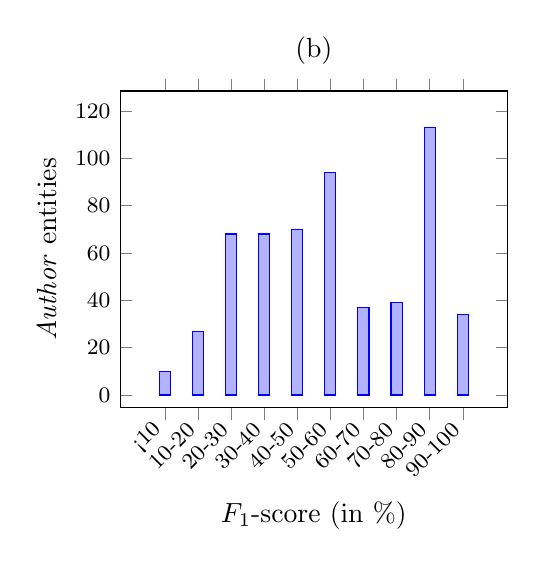
\begin{tikzpicture}[baseline=0]
        \begin{axis}[
        ybar,
        enlargelimits=0.15,
              %legend style={at={(0.5,-0.15)}, anchor=north,legend columns=-1},
        bar width=4,
        ylabel={\textit{Author} entities},
        xlabel={$F_1$-score (in \%)},
        title=(b),
        symbolic x coords={<10, 10-20, 20-30, 30-40, 40-50, 50-60, 60-70, 70-80, 80-90, 90-100},
        xtick=data,
        nodes near coords align={vertical},
        x tick label style={rotate=45,anchor=east},
        ]
        \addplot coordinates {(<10,10)
                              (10-20,27)
                              (20-30,68)
                              (30-40,68)
                              (40-50,70)
                              (50-60,94)
                              (60-70,37)
                              (70-80,39)
                              (80-90,113)
                              (90-100,34)};
        \end{axis}
      \end{tikzpicture}


 \\ %\hline
\end{tabular}
\caption{(a) \textsc{msag} cleaning: Recall and F1 values; (b) \textsc{msag} Experiments} 
\label{tab:msag}
\end{table*}

We extend the applicability of Markov logic to web data and provide initial results on cleaning the highly imperfect graph structured \textsc{MSAG} dataset. We study the efficiency of data cleaning on web data by leveraging the connection between information completeness and data consistency. These two data issues interact with each other: missing values imputation helps to fix inconsistencies, and by correcting values, we identify missing entities. 

In this experiment, we partition our data and run inference for each author in isolation. We obtain a subgraph per \textit{Author}-entity with at least 10 \textit{Paper}-\textit{Author} edges. Next, we randomly select 600 \textit{Author}-entities. 

Table~\ref{tab:msag} (a) shows the accuracy of our approach on the sample of \textsc{MSAG} dataset. We show the accuracy as relation between recall ($x$-axis) and $F_1$-score ($y$-axis). We distinguish between three kinds of \textit{Author}-nodes (which are marked separately in Table~\ref{tab:msag} (a)): 
nodes with one or two missing \textit{Author}-\textit{Organization} edges, nodes with three or four missing values for the \textit{Author} \textit{Organization} connection, and finally nodes with more than 5 missing edges. Additionally, Table~\ref{tab:msag} (b) provides another perspective on this experiment by revealing the exact distribution of corrected \textit{Author}-entities ($x$-axis) by $F_1$-score ($y$-axis). The result shows the following: The method demonstrates overall $F_1$ score greater than $50\%$ and recall greater than $78\%$ for \textit{Author}-entities with one to two missing edges. Starting from three missing edges, we still achieve a recall ranging from $0.8$ to $1.0$, though the precision (and therefore $F_1$ score) drops. This happens because our approach selects more false positives with an increasing number of missing values. This experiment tells us that our method produces satisfying results on web data with very little noise only (e.g., missing values). In future work, extending data cleaning rules with domain specific information should be studied further in order to reduce the false positives rate. We are not able to compare ourselves to another system directly here, because the \textsc{MSAG} dataset has only recently been published and related work in data cleaning systems only provides results for cleaning relational data.

\subsection{Impact of Rule Execution Order}
\label{subsec:exp3}
Next, we study the effects of different orders of data cleaning rule execution, to show that specifying the optimal order of rules manually is hardly achievable~\cite{Dallachiesa:2013:NCD:2463676.2465327}. We investigate whether it is beneficial to leverage joint inference for simultaneous rule execution instead of manual specification of the optimal order of data cleaning rule execution. We verify the result in Figure~\ref{fig:orderexec} by investigating the $F_1$-score ($y$-axis) distribution of various data quality settings executed on varying noise rates ($x$-axis). We run our Markov logic program on the attributes \textsl{state} and \textsl{zip} of the \textsc{hosp} dataset because they both participate in CFD and MD. Furthermore, we fix the dataset size at 90,000 tuples with a noise rate varying from $2\%$ to $10\%$. Each experiment consists of three parts: First, we run the MD rules and then the CFDs, which gives us the overall worst accuracy. This results agree with the previous experiment about the joint modeling data cleaning rules (c.f.,~Table~\ref{tab:plots} (a) and Section~\ref{subsec:exp1}). The MD rules perform poorer than CFDs. The overall $F_1$ score ranges between $0.01$ and $0.02$, which we explain by low precision and recall values due to error propagation from MDs to CFDs.  
In the second part of the experiment, we change the sequence of execution to running CFD rules before MD rules. This slightly improves the $F_1$ scores by increasing them from $0.1$ to $0.3$ for different noise values. We attribute this to the fact that CFDs initially detect more violations. However, analogous to the previous part, error propagation leads to unsatisfactory results. 

In the third and final part of the experiment, we perform the simultaneous execution of CFD and MD rules, where we model matching (for values deduplication) and repair (for erroneous values) processes together. Here we see a rapid increase of all accuracy values from $0.86$ for $2\%$ noise to $0.95$ on $10\%$ noise in comparison to the previously performed sequential execution of data cleaning rules. The growing trend of the $F_1$ scores has the same explanation as the results of the experiment about holistic data cleaning (c.f.,~Table~\ref{tab:plots} (a) and Section \ref{subsec:exp1}): namely the functionality of the CPI algorithm. These results confirm our hypotheses that it is highly beneficial to execute multiple data cleaning rules simultaneously.  

The \textsc{nadeef} system~\cite{Dallachiesa:2013:NCD:2463676.2465327}, which also treats various types of rules holistically, ran an analogous experiment. Note that, on data with $10\%$ noise, we improve the $F_1$-score by $10\%$ over the values reported by \textsc{nadeef}. 

\makeatletter
\let\percent\@percentchar
\makeatother
%\usetikzlibrary{patterns}

\begin{figure}
\centering
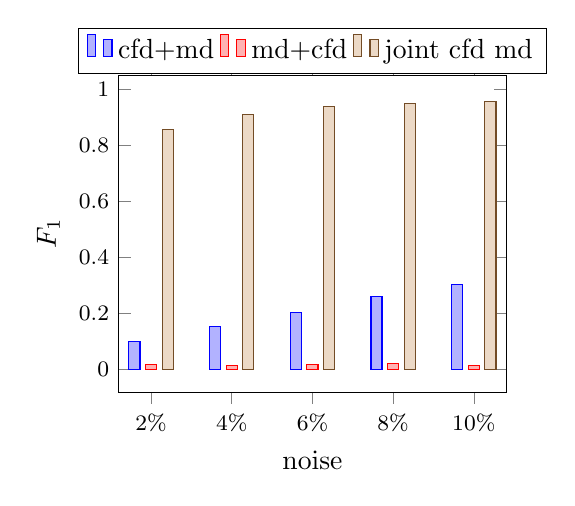
\begin{tikzpicture} 
\begin{axis}[
ybar,
enlargelimits=0.1,
legend style={at={(0.5,1.15)}, anchor=north, legend columns=-1},
bar width=4,
ylabel={$F_1$},
xlabel=noise,
symbolic x coords={{$2\percent$},{$4\percent$},{$6\percent$},{$8\percent$},{$10\percent$}},
xtick=data,
nodes near coords align={vertical},
]
\addplot coordinates {({$2\percent$}, 0.1) ({$4\percent$}, 0.1552) ({$6\percent$}, 0.2039) ({$8\percent$}, 0.2625) ({$10\percent$}, 0.3048)};
\addplot coordinates {({$2\percent$}, 0.0176) ({$4\percent$}, 0.0139) ({$6\percent$}, 0.0173) ({$8\percent$}, 0.0214) ({$10\percent$}, 0.016)};
\addplot coordinates {({$2\percent$}, 0.8566) ({$4\percent$}, 0.9114) ({$6\percent$}, 0.9403) ({$8\percent$}, 0.9512) ({$10\percent$}, 0.9569)};

%\addplot[pattern=north east lines] coordinates {({$2\percent$}, 0.1) ({$4\percent$}, 0.1552) ({$6\percent$}, 0.2039) ({$8\percent$}, 0.2625) ({$10\percent$}, 0.3048)};
%\addplot[pattern=dots] coordinates {({$2\percent$}, 0.0176) ({$4\percent$}, 0.0139) ({$6\percent$}, 0.0173) ({$8\percent$}, 0.0214) ({$10\percent$}, 0.016)};
%\addplot[pattern=horizontal lines] coordinates {({$2\percent$}, 0.8566) ({$4\percent$}, 0.9114) ({$6\percent$}, 0.9403) ({$8\percent$}, 0.9512) ({$10\percent$}, 0.9569)};

\legend{cfd+md,md+cfd,joint cfd md}

\end{axis}
\end{tikzpicture}
\caption{Execution order with Markov Logic} 
\label{fig:orderexec}
\end{figure}

%\subsection{Performance}



\subsection{Modeling Data Cleaning Rules}
\label{subsec:exp4}
%Big table containing all the rules and formulas:
\begin{table*}[t]\footnotesize
\scriptsize
\centering

\begin{tabular}{cll}
\textbf{\textit{Dataset}}               & \multicolumn{1}{c}{\textbf{\textit{Data Cleaning Rules}}}              & \multicolumn{1}{c}{\textbf{\textit{Markov Logic Formulae}}} \\ \hline
%hosp
\multirow{2}{*}{\textsc{hosp}}  & %hosp dq rules
                        \begin{tabular}[c]{@{}l@{}}
                        $\mathsf{cfd_1: \textsc{hosp}([\textsl{zip}] \rightarrow [\textsl{state, city}], t1=(\_ \parallel \_, \_))}$\\
                        %$\mathsf{cfd_2: \textsc{hosp}([\textsl{phone}] \rightarrow [\textsl{addr, city}],t2=(\_ \parallel \_,\_,\_,\_))}$
                        \end{tabular}                   
                        & %hosp markov logic cfd
                        \begin{tabular}[c]{@{}l@{}}
                        $\mathsf{w_1: \textsl{zip/\textsc{hosp}}(id1, code)~\wedge~\textsl{zip/\textsc{hosp}}(id2, code)~\wedge }$\\
                        $\mathsf{~~~~~~~~\textsl{state/\textsc{hosp}}(id1, s1)~\wedge~\textsl{state/\textsc{hosp}}(id2, s2)~\wedge}$ \\
                        $\mathsf{~~~~~~~~!\textsl{state/\textsc{hosp}}(id1, s2)~\wedge~!\textsl{state/\textsc{hosp}}(id2, s1)~\Rightarrow \textsl{equal-state/\textsc{hosp}}(id1, id2)}$\\
                        %second cfd:
                        $\mathsf{w_2: \textsl{zip/\textsc{hosp}}(id1, code)~\wedge~\textsl{zip/\textsc{hosp}}(id2, code)~\wedge }$\\
                        $\mathsf{~~~~~~~~~\textsl{city/\textsc{hosp}}(id1, c1)~\wedge~\textsl{city/\textsc{hosp}}(id2, c2)~\wedge}$ \\
                        $\mathsf{~~~~~~~~~!\textsl{city/\textsc{hosp}}(id1, c2)~\wedge~!\textsl{city/\textsc{hosp}}(id2, c1)~\Rightarrow \textsl{equal-city/\textsc{hosp}}(id1, id2)}$
                        \end{tabular}                 \\ 
                       & %hosp md rule
                         \begin{tabular}[c]{@{}l@{}}
                        $\mathsf{md_1: \textsc{hosp}[\textsl{zip}]=\textsc{zipcode}[\textsl{zip}]\wedge \textsc{hosp}[\textsl{state}]\neq \textsc{zipcode}[\textsl{state}]}$\\
                        $\mathsf{~~~~~~~~~~~~~~\rightarrow\textsc{hosp}[\textsl{state}]\rightleftharpoons \textsc{zipcode}[\textsl{state}]} $
                        \end{tabular}                 
                       & %hosp markov logic md
                       \begin{tabular}[c]{@{}l@{}}
                        $ \mathsf{w_3: \textsl{zip/\textsc{hosp}}(id1, code)~\wedge~\textsl{zip/\textsc{ZipCode}}(id2, code)~\wedge }$\\
                        $\mathsf{~~~~~~~~~\textsl{state/\textsc{hosp}}(id1, s1)~\wedge~\textsl{state/\textsc{ZipCode}}(id2, s2)~}$ \\
                        $\mathsf{~~~~~~~~~\Rightarrow \textsl{\textsc{hosp}/match-State/\textsc{ZipCode}}(id1, id2)} $
                       \end{tabular}                  
                       \\ \hline

%tpc-h
\multirow{2}{*}{\textsc{tpc-h}} & %tpc-h fds
                        \begin{tabular}[c]{@{}l@{}}
                        $\mathsf{cfd_1: \textsc{t}([\textsl{c\_custkey}] \rightarrow [\textsl{c\_name,c\_address}],t1=(\_ \parallel \_, \_))} $
                        \end{tabular}                   
                        &%tpc-h mlogic fds
                         \begin{tabular}[c]{@{}l@{}}
                        $ \mathsf{w_1: \textsl{custKey}(id1, key) \wedge \textsl{custKey}(id2, key) \wedge }$\\
                        $\mathsf{~~~~~~~~~\textsl{name}(id1, n1) \wedge \textsl{name}(id2, n2) \wedge~}$\\
                        $\mathsf{~~~~~~~~~!\textsl{name}(id1, n2)\wedge~!\textsl{name}(id2, n1) \Rightarrow \textsl{equal-Names}(id1, id2)} $\\
                        %second cfd
                        $ \mathsf{w_2: \textsl{custKey}(id1, key) \wedge \textsl{custKey}(id2, key) \wedge }$\\
                        $\mathsf{~~~~~~~~~\textsl{addr}(id1, addr1) \wedge \textsl{addr}(id2, addr2) \wedge~}$\\
                        $\mathsf{~~~~~~~~~!\textsl{addr}(id1, addr2)\wedge~!\textsl{addr}(id2, addr1) \Rightarrow \textsl{equal-Names}(id1, id2)} $
                        \end{tabular}                    
                         \\  
                       & %tpch md rules
                       \begin{tabular}[c]{@{}l@{}}
                        $\mathsf{md_1: \textsc{t}[\textsl{c\_address}]=\textsc{t}[\textsl{c\_address}] \rightarrow \textsc{t}[\textsl{c\_phone}]\rightleftharpoons \textsc{t}[\textsl{c\_phone}]}$\\ 
                        %$\mathsf{md_2: \textsc{t}[\textsl{c\_name}]=\textsc{t}[\textsl{c\_name}] \rightarrow \textsc{t}[\textsl{c\_address}]\rightleftharpoons \textsc{t}[\textsl{c\_address}]} $

                        \end{tabular}                  
                       & %tpch md markov logic
                       \begin{tabular}[c]{@{}l@{}}
                        $\mathsf{w_3: \textsl{addr}(id1, addr) \wedge \textsl{addr}(id2, addr) \wedge~}$\\
                        $\mathsf{~~~~~~~~~\textsl{phone}(id1, phone1) \wedge \textsl{phone}(id2, phone2) \wedge~}$\\
                        $\mathsf{~~~~~~~~~ \Rightarrow  \textsl{match-Phone}(id1, id2)} $
                        \end{tabular}                     
                       \\ \hline
%msag
\multirow{3}{*}{\textsc{msag}}  & % msag fd
                                \begin{tabular}[c]{@{}l@{}}
                                $\mathsf{cfd_1: \textsc{m}([\textsl{author\_id, year}] \rightarrow [\textsl{affiliation\_id}],t1=(\_,\_ \parallel \_))} $\\
                                %$\mathsf{cfd_2: \textsc{m}([\textsl{affiliation\_id}] \rightarrow [\textsl{origin\_name}],t2=(\_ \parallel \_))} $
                                \end{tabular}                   
                                & %msag markov logic fd
                                \begin{tabular}[c]{@{}l@{}}
                                $\mathsf{w_1: \textsl{author}(pid1,aid1)\wedge\textsl{author}(pid2,aid2)\wedge }$\\
                                $\mathsf{~~~~~~~~~\textsl{publishYear}(pid1,y)\wedge\textsl{publishYear}(pid2,y)\Rightarrow \textsl{equal-Affiliation}(pid1, pid2)}$\\
                                \end{tabular}                   
                                \\  
                                & % msag extended fd
                                \begin{tabular}[c]{@{}l@{}}
                                 $\mathsf{eCfd_1: \textsc{m}([\textsl{author\_id, year}] \rightarrow [\textsl{affiliation\_id}],}$\\
                                 $\mathsf{~~~~~~~~~t1=(\_, diff(\_)\leq 2 \parallel \_))} $   
                                \end{tabular}             
                                & % msag markov logic 
                                \begin{tabular}[c]{@{}l@{}}
                                $\mathsf{w_2: \textsl{author}(pid1,aid1)\wedge\textsl{author}(pid2,aid2)\wedge }$\\
                                $\mathsf{~~~~~~~~~\textsl{publishYear}(pid1,y1)\wedge\textsl{publishYear}(pid2,y2)\wedge }$\\
                                $\mathsf{~~~~~~~~~\textsl{inRange}(y1, y2)\Rightarrow \textsl{equal-Affiliation}(pid1, pid2)}$\\
                                \end{tabular}  
                                \\
                                &%additional predicates for msag
                                %nothing here
                                & %Equality axioms:
                                \begin{tabular}[c]{@{}l@{}}
                                $symmetry:$\\
                                $\mathsf{\infty:~\textsl{equal-Affiliation}(pid1, pid2)\Rightarrow \textsl{equal-Affiliation}(pid2, pid1)}$\\
                                $transitivity:$\\
                                $\mathsf{\infty:~\textsl{equal-Affiliation}(pid1, pid2)\wedge \textsl{equal-Affiliation}(pid2, pid3)}$\\
                                $\mathsf{~~~~~~~~~\Rightarrow \textsl{equal-Affiliation}(pid1, pid3)}$\\
                                \end{tabular}  

                                \\ \hline
\end{tabular}
\caption{Modeling data cleaning rules as Markov logic programs.}
\label{tab:rulesformulas}
\end{table*}

%\note{This section would greatly benefit from a few concrete examples that show the benefits of modeling rules with markov logic!!! Furthermore, you need to explain how you measure usability!!!} - due to space limitations, I extracted all examples into a table. 
%\note{trying to elaborate the usability methodology from} \cite{Lewis2013UMUX, Finstad2010}
% http://www.measuringu.com/blog/essential-metrics.php

To assess the usability of our method, we adopt the research methodology from \textsc{umux-lite}~\cite{Lewis2013UMUX, Finstad2010} and discuss two items from the \textsc{umux-lite} questionnaire: "Markov logic capabilities meet the requirements of data cleaning systems" and "Markov logic is easy to use". As explained in the previous Sections \ref{sec:method}, \ref{subsec:exp1}, \ref{subsec:exp2} and \ref{subsec:exp3}, Markov logic meets the main requirements of data cleaning systems such as \textit{holistic} data quality rules treatment \cite{Fan:2014:IRM:2628135.2567657, Dallachiesa:2013:NCD:2463676.2465327}, automation \cite{Stonebraker_datacuration} and heterogeneous rules incorporation \cite{chu2013holistic}. In the following, we focus on the second item from \textsc{umux-lite} - "Markov logic is easy to use" - and provide our experience in how we modeled data cleaning rules by using Markov logic on all three datasets \textsc{hosp}, \textsc{tpc-h} and \textsc{msag}. %Table \ref{tab:rulesformulas}

\textbf{\textsc{hosp} Quality Rules}. In our data cleaning method for the \textsc{hosp} data, we use 6 manually designed CDFs and one MD, which result in 15 normalized CFDs. One MD rule is transformed into 2 formulas. All data cleaning rules are positive. Finally, all interleaved rules are translated into 21 Markov logic formulas. In Table~\ref{tab:rulesformulas}, we provide an example of these data quality rules, which are defined on pairs of tuples. The MD rule is specified on two relations. Markov logic predicates used for data quality formulas are shown in Table~\ref{tab:predicates}. After transforming the 100k \textsc{hosp} tuples into Markov logic grounded atoms, the resulting data comprises 1.3M evidence atoms, which are used for inference. We empirically observe that extending the data quality rules set for additional conditions makes consideration of similar tuples unnecessary and reduces the search space and therefore converges much faster than the \textit{"pure"} model. This means that each first order logic formula, which represents the RHS of the normalized data quality rule $\mathsf{\textsl{attr}(id1, v1)~\wedge~\textsl{attr}(id2, v2)}$, becomes an inverse part $\mathsf{!\textsl{attr}(id1, v2)~\wedge~!\textsl{attr}(id2, v1)}$. This additional part denotes that we consider only tuples with different values. Here the normalized CFD rules are being compiled as demonstrated in the Table \ref{tab:rulesformulas}. 
%\note{What has this whole paragraph to do with usability? How did you measure it? What is the purpose of this discussion?}

\textbf{\textsc{tpc-h} Quality Rules}. We write 9 CFDs and 3 MDs for this dataset. One example of the rules is a CFD that states if two tuples match on \textsl{c\_custkey}, then they should match on the \textsl{c\_name} and \textsl{c\_address} attributes. MDs are designed on the same schema \textsc{tpc-h} \textsl{(T, T)}. These MDs state that if the LHS is similar for any pair of tuples $(t_1,t_2)$, then the attribute values on the RHS should be identified. We provide an except of the data quality rules we created for \textsc{tpc-h} in Table~\ref{tab:rulesformulas}. Table~\ref{tab:predicates} shows the Markov logic predicates which we use for data quality rules. After transforming the 100k \textsc{tpc-h} tuples into Markov logic grounded atoms, the resulting data comprises 1 Mio evidence atoms, which are leveraged by the inference. 
%\note{Again: What has this whole paragraph to do with usability? How did you measure it? What is the purpose of this discussion?}

\textbf{\textsc{msag} Quality Rules}. Due to the graph nature of the \textsc{msag} data (c.f.,~Figure \ref{fig:msagmissing}), we develop data quality rules, which are based on CFDs, \textit{extended} CFDs \cite{Chen2009extended}, and equality axioms, such as \textit{symmetry} and \textit{transitivity}. For the \textit{Paper}-\textit{Author}-\textit{Organization} subgraph we define two CFDs, one extended CFD and 8 additional rules that comprises equality axioms for hidden predicates. Considering the semantical meaning of the data, we profit from the ability to add supporting knowledge into the data cleaning process. For example, the CFD $\mathsf{\textsc{m}([\textsl{author\_id, year}] \rightarrow [\textsl{affiliation\_id}],t1=(\_,\_ \parallel \_))} $ allows us to capture all missing affiliations by the same author, which published in the same year. In real life, we know that in academia an average contract lasts around 2-3 years. Therefore we will extend our search range by incorporating this knowledge in the form of a predicate $\mathsf{\textsl{inRange}(year, year)}$. Additionally we enable capturing more missing values by adding equality axioms. For example, the hard rule $\mathsf{\textsl{equal-Affiliation}(id_1, id_2) ~\wedge~ \textsl{equal-Affiliation}}$ $\mathsf{(id_2, id_3) \Rightarrow  \textsl{equal-Affiliation}(id_1, id_3)}$ denotes a transitive relationship between three different entities \textit{Organization}. In total, our Markov logic program then consists of 21 lines of code (we provide an excerpt in Table~\ref{tab:rulesformulas}). 
%\note{Again: What has this whole paragraph to do with usability? How did you measure it? What is the purpose of this discussion?}

This part of our experimental study demonstrates how the expressiveness of Markov logic enables us to model data cleaning rules. While existing data cleaning systems \cite{Dallachiesa:2013:NCD:2463676.2465327} are also concerned about the generality of the data cleaning rules, we define Markov logic data cleaning rules in expressive first-order logic manner without the need to implement any code. Furthermore, Markov logic is data format independent, which facilitates data cleaning on different data formats (e.g., on relational and graph data formats). 

\subsection{Summary}
The results of our experimental study indicate that multiple types of data cleaning rules should be considered \textit{holistically} (c.f.,~Section~\ref{subsec:exp1} and \ref{subsec:exp2}), which confirms previous research \cite{Dallachiesa:2013:NCD:2463676.2465327, Fan:2014:IRM:2628135.2567657, Fan:2011:IRM:1989323.1989373}. Adding domain or structural knowledge about data into the Markov logic program improves the quality of data cleaning. Furthermore, joint inference enables us to achieve highly satisfactory results without having to define the order of the execution of the data cleaning rules. We find that joint modeling of data quality rules results in higher accuracy of data correction~(c.f.,~Section \ref{subsec:exp3}). By using the probabilistic-logical framework of Markov logic, we benefit from its flexibility in constraint definition and joint inference over different data repair and matching rules. The direct translation of data cleaning rules into first-order logic (Markov logic formulas) simplifies the process of writing data cleaning routines (c.f.,~Section~\ref{subsec:exp4}). 
